% !TEX root = Bachelorarbeit_Paul_Zilewitsch.tex
\section{Konzipierung}

\subsection{Vorbetrachtung}
\noindent
Für die Erstellung einer Meldung sind mehrere Informationen bzw. Eigenschaften nötig. Dabei sind einige Informationsangaben Pflichtfelder in der Benutzeroberfläche von GEBman 10. Füllt der Benutzer diese nicht aus, kann keine neue Meldung erstellt werden. Die Tabelle~\ref{tab:Medlungseigenschaften} zeigt nun einige Eigenschaften, die für die spätere Erstellung einer Meldung im Programmcode wichtig sein werden.

\begin{table}[h!]
    \begin{tabular}{ | l | p{11cm}|}
    \hline
    Bezeichnung & Erläuterung \\ \hline
 * Art & Hier muss die Art der Meldung angegeben werden. Ist es beispielsweise eine Störmeldung oder eine Servicemeldung. \\ \hline
 * Status & Dieses Pflichtfeld ist standardmäßig auf \enquote{unbearbeitet} gestellt.  \\ \hline
* Standort oder Objekt & Eines der beiden Felder muss ausgefüllt sein, um die Meldung einem Standort oder einem Objekt zuweisen zu können. \\ \hline
* Meldung & Das ist das wichtigste Feld, denn hier wird kurz beschrieben, welcher Vorfall sich ereignet hat. \\ \hline
Beschreibung & Für eine genauere Beschreibung des Vorfalls ist dieses Feld vorgesehen und bietet hierfür ausreichend Platz. \\ \hline
    \end{tabular}
    \caption[Einige Eigenschaften für eine Meldung]{Einige Eigenschaften für eine Meldung, Quelle: eigene Darstellung}
    \label{tab:Medlungseigenschaften}
\end{table}

\noindent
Die Eigenschaften mit dem Stern ( * ) als Kennzeichnung sind die erwähnten Pflichtfelder. Bei diesen erforderlichen Eigenschaften ergibt sich ein Problem für die Erstellung einer Meldung über die E-Mail Integration. Derjenige, der eine E-Mail an den Exchange Server von GEBman 10 schreibt, müsste eine genaue Angabe über den Standort und/oder das Objekt der Meldung machen. Das ist in der Praxis nicht bedienerfreundlich und könnte zu Schreibfehlern führen. Auf der Seite der Implementierung hieße das, dass ein möglicher Schreibfehler abgefangen werden muss, da dieser Standort oder diese Objekte nicht in der Datenbank existieren. Außerdem hatten bereits mehrere Kunden von der KMS Computer GmbH dieses Pflichtfeld als nicht hilfreich bezeichnet. Will der Kunde einfach nur Meldungen in dem Service Desk Modul aufgeben, ist diese Eigenschaft unnütz. Aus diesen Gründen wurde entschieden, die Felder Standort und Objekt nicht mehr als notwendige Eigenschaften einer Meldung zu definieren. Dadurch werden diese beiden Eigenschaften in der Implementierung auch weiter beachtet und der Service Desk wird weiter vom Facility Management Bereich gelöst. \newline
Die Informationsangabe Beschreibung ohne den Stern sind nicht verpflichtend, ist aber durchaus sinnvoll bei der Erstellung einer Meldung. Es gibt noch weitere Felder, die der Benutzer in der Benutzeroberfläche ausfüllen kann, die aber nicht verpflichtend sind. Diese zusätzlichen Informationen sind für die nachfolgenden Ausführungen nicht relevant.

\subsection{Zielsetzung und Grundidee Module Service }
\noindent
Ausgangspunkt ist ein Benutzer, der Mails an den Exchange Server schreiben kann, um somit neue Meldungen im Service Desk Modul anzulegen. Alle E-Mails, die an den Exchange Server gesendet werden, landen im Posteingang des Exchange Servers. Ziel ist es, durch das Auswerten dieser im Posteingang befindlichen E-Mails, Meldungen zu erstellen, ohne dass sich ein Benutzer in GEBman 10 anmelden muss. Der Benutzer soll somit eine neue Meldung erstellen, auf eine vorhandene Meldung antworten können. Hierfür ist eine ID notwendig, die jeder neuen Meldung zugeteilt wird. Sollte der Benutzer einer Meldung eine Antwort hinzufügen wollen, muss die ID der Meldung im Betreff der E-Mail stehen. Demzufolge ist der Betreff einer E-Mail entscheidend für das weitere Vorgehen im Programmcode. Außerdem soll es möglich sein, mögliche E-Mail Anhänge direkt an die Meldung zu binden. In GEBman 10 hat jede Meldung bereits einen Bereich für Dokumente. So kann über den Programmcode dieser Bereich mit durch mögliche E-Mail Anhänge erweitert werden. \newline 
In GEBman 10 ist eine Klasse Module Service implementiert, die es ermöglicht, einen Service asynchron vom restlichen System für das entsprechende Modul laufen zu lassen. Demnach muss in GEBman 10 ein neuer Service erstellt werden, der in bestimmten Intervallen seine Funktion ausführt. Das geschieht im Code im Package Common. In diesem zentralen Package werden Funktionalitäten implementiert, die für alle Module allgemein gültig sind. Dadurch kann die Erweiterung später auch für andere Module verwendet werden und nicht nur im Service Desk Modul.\newline
Nach dem Auswerten der E-Mails im Packge Common muss im Modul Service Desk eine Meldung erstellt oder bearbeitet werden. Das heißt, dass diese Funktionalität im Package Service Desk implementiert werden sollte. Hier befinden sich alle Komponenten, die auf die Meldungen in GEBman 10 zugreifen. Nach der erfolgreichen Erstellung einer neuen Meldung soll der Benutzer eine Bestätigungsmail erhalten. Hierfür können die bereits vorhandenen Funktionalitäten als Grundlage genutzt werden.\newline
Um diese Grundidee besser erläutern und umsetzen zu können, ist eine Darstellung der einzelnen Schritten in verschiedenen UML-Diagrammen sinnvoll.

\newpage


\subsection{UML - Modellierung}
\noindent
Grundlage der Modellierung bildet die grafische Notation Unifed Modeling Language (UML) in der Version 2.3. UML hat sich in den letzten Jahren bei der Erstellung objektorientierter Modelle bewährt und ermöglicht somit einheitliche Diagrammdarstellungen und Begriffsabgrenzungen. Deshalb kann UML als Standard für die Modellierung objektorientierter Software gesehen werden.\footnote{Vgl. \citeauthor{Schneider} (\citeyear{Schneider}), S. 233.}\footnote{Vgl. \citeauthor{Balzert} (\citeyear{Balzert}), S. V.}\\\\
Grundsätzlich werden zwei Sichtweisen in der UML unterschieden. Die nachfolgende Tabelle erläutert die wichtigsten Unterschiede:

\begin{table}[h!]
    \begin{tabular}{ | p{2.5cm}| p{6cm} | p{6cm} |}
    \hline
    Diagrammtyp & Verhaltensdiagramm & Strukturdiagramm \\ \hline
   Sichtweise & dynamisch & statisch \\ \hline
   Beispiele & Aktivitätsdiagramm, Zustandsdiagramm, Sequenzdiagramm &  Klassendiagramm, 
   Objektdiagramm, Paketdiagramm\\ \hline
   Beschreibung &  Es werden die Komponenten des Systems erläutert, die sich während der Laufzeit 
   verändern. Dabei werden die Abläufe des Systems ersichtlich und auch inwiefern der Benutzer diese 
   beeinflusst & Aus dieser Sicht werden die Komponenten des Systems betrachtet, die unabhängig von 
   der Laufzeit sind. Ihre Ein-und Ausgabedaten können sich verändern, aber die Beziehungen zwischen 
   den Komponenten bleiben bestehen. \\ \hline  
    \end{tabular}
    \caption[UML-Diagrammtypen]{UML-Diagrammtypen, Quelle: in Anlehnung an Schneider (2012) , S. 234.}
\end{table}


\noindent
Insgesamt gibt es sieben Verhaltens -und sieben Strukturdiagramme. Es können nicht alle vierzehn Diagramme in dieser Arbeit Platz finden und bei einem solchen Vorgehen würde auch der Fokus auf die wichtigsten Fragestellungen verloren gehen. Aus diesem Grund wurden zwei Verhaltensdiagramme und ein Strukturdiagramm ausgewählt, die die Abläufe bei der Erweiterung des Service Desk von GEBman 10 ersichtlich machen und die Implementierung erleichtern sollen. \\

\noindent
Das erste Verhaltensdiagramm soll die Frage klären, welche Aktionen der Benutzer mit dem Versenden einer E-Mail ausführen kann und wie das System darauf reagiert. Im Punkt 4.2 wurde auf die Anforderungen der Erweiterung eingegangen. Diese werden nun mit dem Aktivitätsdiagramm  in der Abbildung~\ref{fig:Aktivitaetsdiagramm} erläutert.

\begin{figure}[h!]
\centering
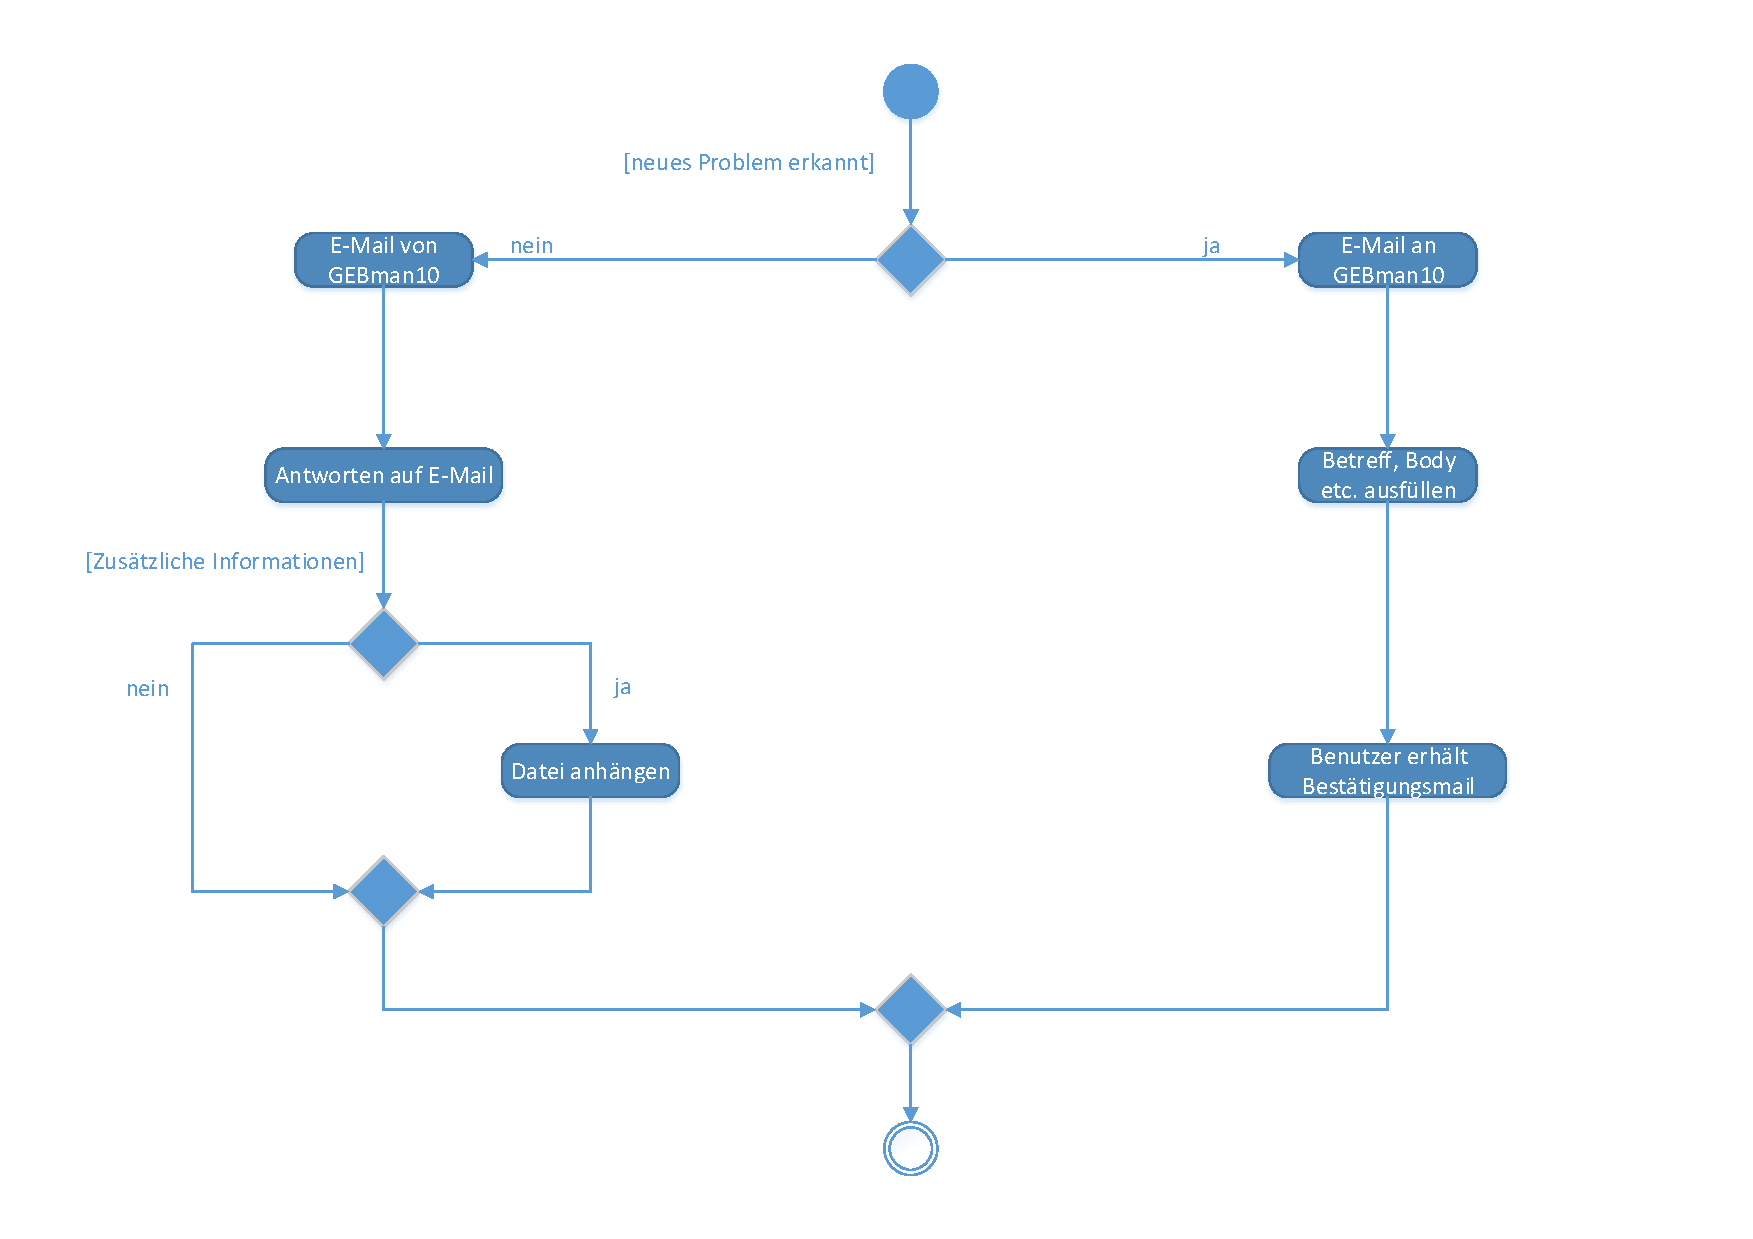
\includegraphics[width=0.80\textwidth]{Abbildungen/Aktivitaetsdiagramm.pdf}
	\caption[Aktivit{\"a}tsdiagramm]{Aktivit{\"a}tsdiagramm, Quelle: eigene Darstellung}
	\label{fig:Aktivitaetsdiagramm}
\end{figure}

\noindent
Der Benutzer muss sich direkt zu Beginn entscheiden, ob er eine neue Meldung erstellen oder auf eine bestehende Meldung antworten möchte. Sollte er ein neues Problem erkannt haben, schickt er eine E-Mail an GEBman 10. Im Betreff muss die Meldung eingetragen werden und im Textkörper der E-Mail kann der Benutzer die ausführliche Beschreibung des Problems angeben. Der ModulService in  GEBman 10 wertet diese E-Mail aus und legt eine neue Meldung im Service Desk an. Diese Meldung erhält eine eindeutige ID. Der Benutzer erhält anschließend eine Bestätigungsmail mit der ID der Meldung, wenn die Erstellung erfolgreich war.\newline
Möchte der Benutzer allerdings auf bereits bestehende Meldungen antworten, so kann er direkt auf eine E-Mail von GEBman 10 antworten. Der Betreff wird automatisch übernommen und somit ist die ID schon eingetragen. Sollte der Benutzer zusätzliche Informationen wie eine Excel-Tablle oder ein Bild an die Meldung binden wollen, kann er der E-Mail einen Anhang hinzufügen.\\\\

\noindent
Anders als bei dem Aktivitätsdiagramm wird in der nachfolgenden Abbildung ein Zustandsdiagramm dargestellt. Die beiden Diagramme ähneln sich von ihrer Notation sehr. Das Zustandsdiagramm legt den Fokus jedoch auf die Zustände des Systems, die es während der Laufzeit annehmen kann. Deshalb ist es auch das zweite Verhaltensdiagramm. Hierbei ist es wichtig, dass immer ein Ereignis eintreffen muss, damit das System in einen anderen Zustand wechseln kann.\footnote{Vgl. \citeauthor{Balzert} (\citeyear{Balzert}), S. 40.}

\begin{figure}[h!]
\centering
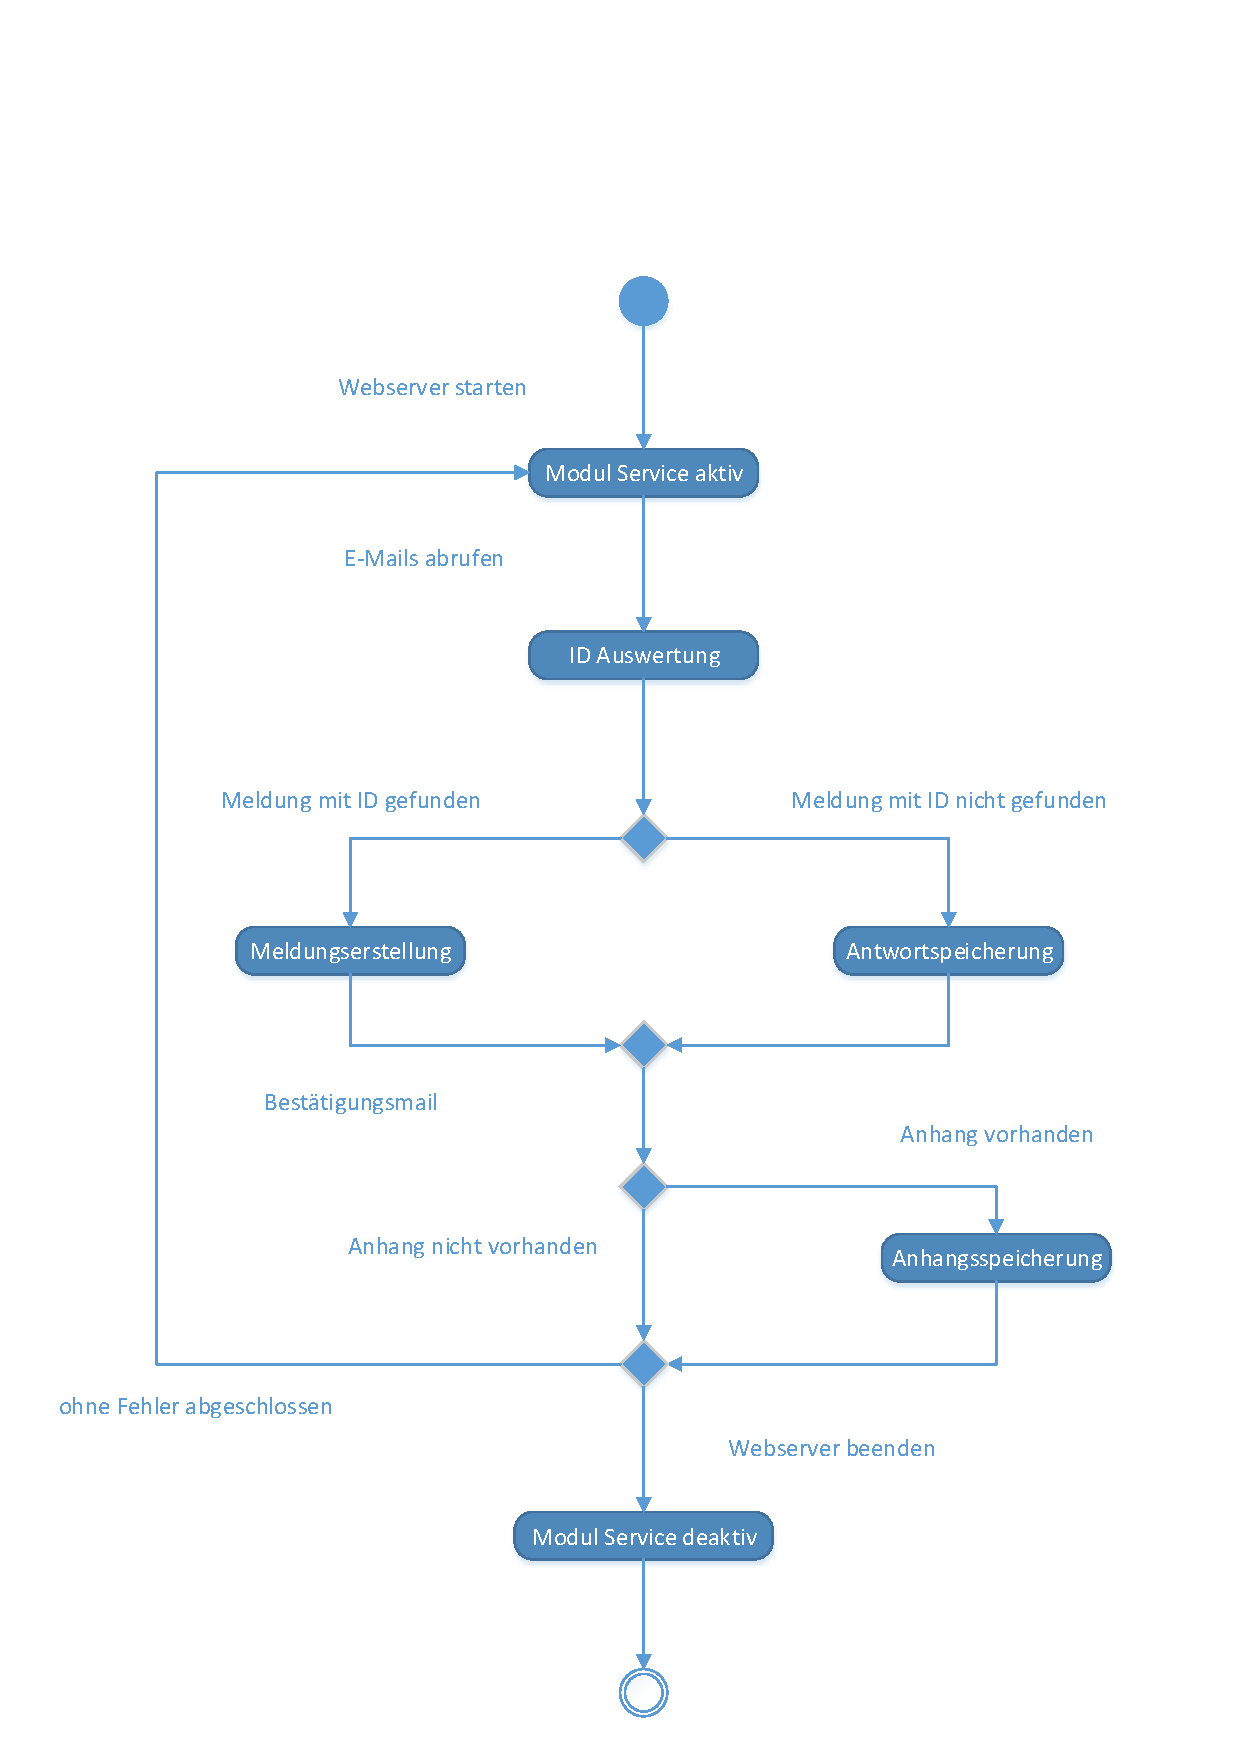
\includegraphics[width=0.6\textwidth]{Abbildungen/Zustandsdiagramm.pdf}
	\caption[Zustandsdiagramm]{Zustandsdiagramm, Quelle: eigene Darstellung}
	\label{fig:Zustandsdiagramm}
\end{figure}

\noindent
Sobald der Webserver gestartet ist, befindet sich das System im Zustand aktiver Module Service. In regelmäßigen Zeitabständen, werden über diesen Service die neuesten Mails von dem Exchange Server geholt. Dann werden die in der Betreffzeile der Mail befindlichen ID's ausgewertet. Ist keine ID vorhanden, geht der Module Service in den Zustand einer neuen Meldungserstellung über. Dabei werden alle nötigen Informationen der E-Mail entnommen. Anschließend wird die Bestätigungsmail versendet, wenn die Erstellung erfolgreich war.\newline
Wurde bei der ID Auswertung allerdings festgestellt, dass eine Meldung mit identischer ID vorhanden ist, wechselt das Sytem in den Zustand der Antworterstellung. Hier wird der Textkörper der E-Mail als Antwort der Meldung hinzugefügt.\newline
Nachdem eines der beiden Szenarien abgearbeitet wurde, kann das System noch in den Zustand der Anhangsspeicherung gelangen. In diesem Zustand wird dann der Anhang der E-Mail an die Meldung gebunden. Wurden alle Prozesse ohne Fehler abgeschlossen, kehrt das System wieder zu dem Anfangszustand es aktiven Webservice zurück. Der Modul Service wird dann im nächsten Intervall die Prozedur wiederholen. Nur wenn der Webserver beendet wird, ist logischerweise auch der Module Service deaktiviert. Ansonsten wird der Service permanent laufen.\\\\

\noindent
Die Verhaltensdiagramme aus Benutzer -und Systemperspektive sind somit abgeschlossen. Das Klassendiagramm in Abbildung~\ref{fig:Klassendiagramm} ist ein Strukturdiagramm, welches einen groben Überblick über den zu implementierenden Module Service und seiner Beziehung zu dem restlichen System geben soll. \newpage 

\begin{figure}[h!]
\centering
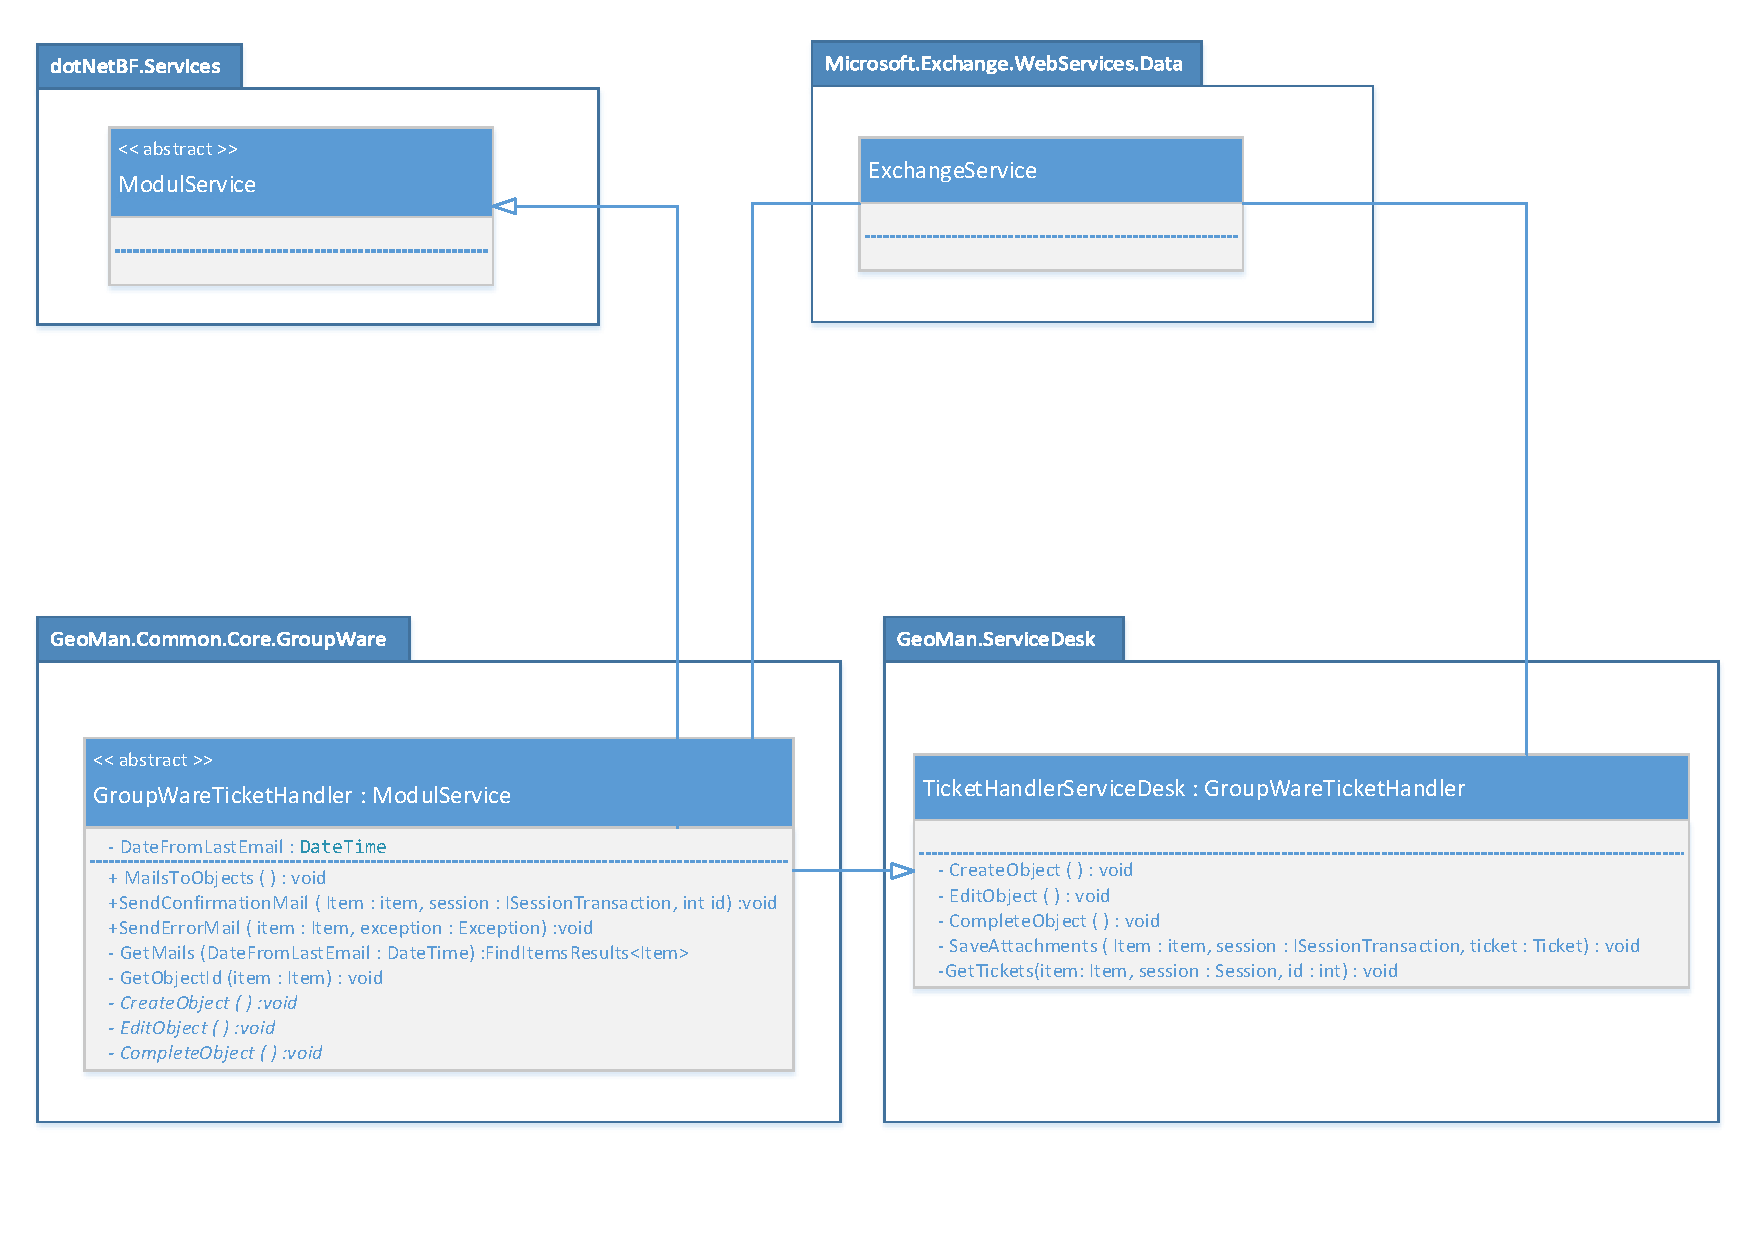
\includegraphics[width=0.80\textwidth]{Abbildungen/Klassendiagramm.pdf}
	\caption[Klassendiagramm]{Klassendiagramm, Quelle: eigene Darstellung}
	\label{fig:Klassendiagramm}
\end{figure}

\noindent
Die Funktionalitäten für das Versenden von E-Mails in GEBman 10 befinden sich im Package \textit{GeoMan.Common.Core.GroupWare}. Die abstrakte Klasse für den Modul Service wird \textit{GroupWareMailToObjectFactory} heißen und sich ebenfalls in diesem Package befinden. Sie erbt von der ebenfalls abstrakten Klasse \textit{ModuleService}, welche sich in einem Framework befindet, das ein Partnerunternehmen der KMS Computer GmbH entwickelt.\\ 

\noindent
\textit{GroupWareMailToObjectFactory} wird nur das öffentliche Attribut \textit{DateFromLastEmail} besitzen. Diese Variable speichert das Ankunftsdatum von der neuesten E-Mail im Exchange Postfach und hat deshalb den Datentypen \textit{DateTime}. Somit müssen nicht alle E-Mails abgerufen werden, sondern nur die, die nach dem Ankunftsdatum der letzten E-Mail eingetroffen sind.\newline
Diese Klasse\textit{GroupWareMailToObjectFactory} wird auf die Exchange Webservices zugreifen und sich Methoden der Klasse Exchange Service bedienen, um die E-Mails von Exchange Server abzufragen. Das übernimmt die Methode \textit{GetMails( )}, die den Zeitpunkt der zuletzt abgerufenen E-Mail als Argument übergeben bekommt. Der Rückgabewert ist eine ItemView vom Exchange Webservice. Deshalb wird eine Referenz auf die Microsoft Exchange Web Services Data benötigt.
\newline 
Die Methode \textit{CheckIdFromMails( )} wird die ID's überprüfen, die in den Betreff der Mails eingetragen wurde. Auch ist sie dafür zuständig, die entsprechenden Methoden für das weitere Vorgehen aufzurufen. Die Methoden \textit{SendConfirmationMail( )} und \textit{SendErrorMail( )} werden dafür zuständig sein, eine Bestätigungsmail oder eine Fehlermail zu versenden, wenn der entsprechende Fall eintritt. Es wird drei abstrakte Methoden geben, die eine Meldung erstellen (\textit{CreateObject}), eine Meldung bearbeiten (\textit{EditObject}) oder den Status einer Meldung ändern (\textit{CompleteObject}). Ihnen wird jeweils die entsprechende Mail als Attribut mitgegeben.\\

\noindent
Die abstrakten Methoden werden dann in der Klasse TicketHandler überschrieben. Erst in dieser Klasse wird es zu der eigentlichen Erstellung, Bearbeitung oder Änderung des Status kommen. Dafür muss die Klasse \textit{TicketHandler} von der abstrakten Klasse \textit{GroupWareMailToObjectFactory} erben. Die Microsoft Web Services werden ebenfalls in der Klasse \textit{TicketHandler} benötigt, da erst hier die Parameter wie E-Mail-Body oder Recipient ausgewertet werden.\\


\subsection{Sicherheitsaspekte}
\noindent
Immer wieder vernachlässigen Entwickler die Sicherheit ihrer Implementierungen.\footnote{Vgl. \citeauthor{Ziegler} (\citeyear{Ziegler}), S. 53.}\footnote{Website: \citeauthor{Sicherheit} (abgerufen am: 23.06.2016)} Das liegt häufig an mangelnder Zeit, da Releases einen festen Zeitplan verfolgen, den es einzuhalten gilt. Es kann aber auch sein, dass die Implementierung nicht aus dem Blickwinkel der Sicherheit betrachtet wird und der Fokus eher auf Bereiche wie Benutzerfreundlichkeit gelegt wird. Natürlich hat das wenig mit Sicherheit zu tun. Dabei können es Entwickler mit wenig Aufwand Angreifern deutlich schwerer machen. Deswegen werden im Nachfolgenden zwei Sicherheitsprobleme für die Umsetzung des Konzepts in GEBman 10 besprochen. Die Abbildung~\ref{fig:Sicherheitsprobleme} zeigt zwei kritische Bereiche, die genauer erläutert werden müssen.

\begin{figure}[h!]
\centering
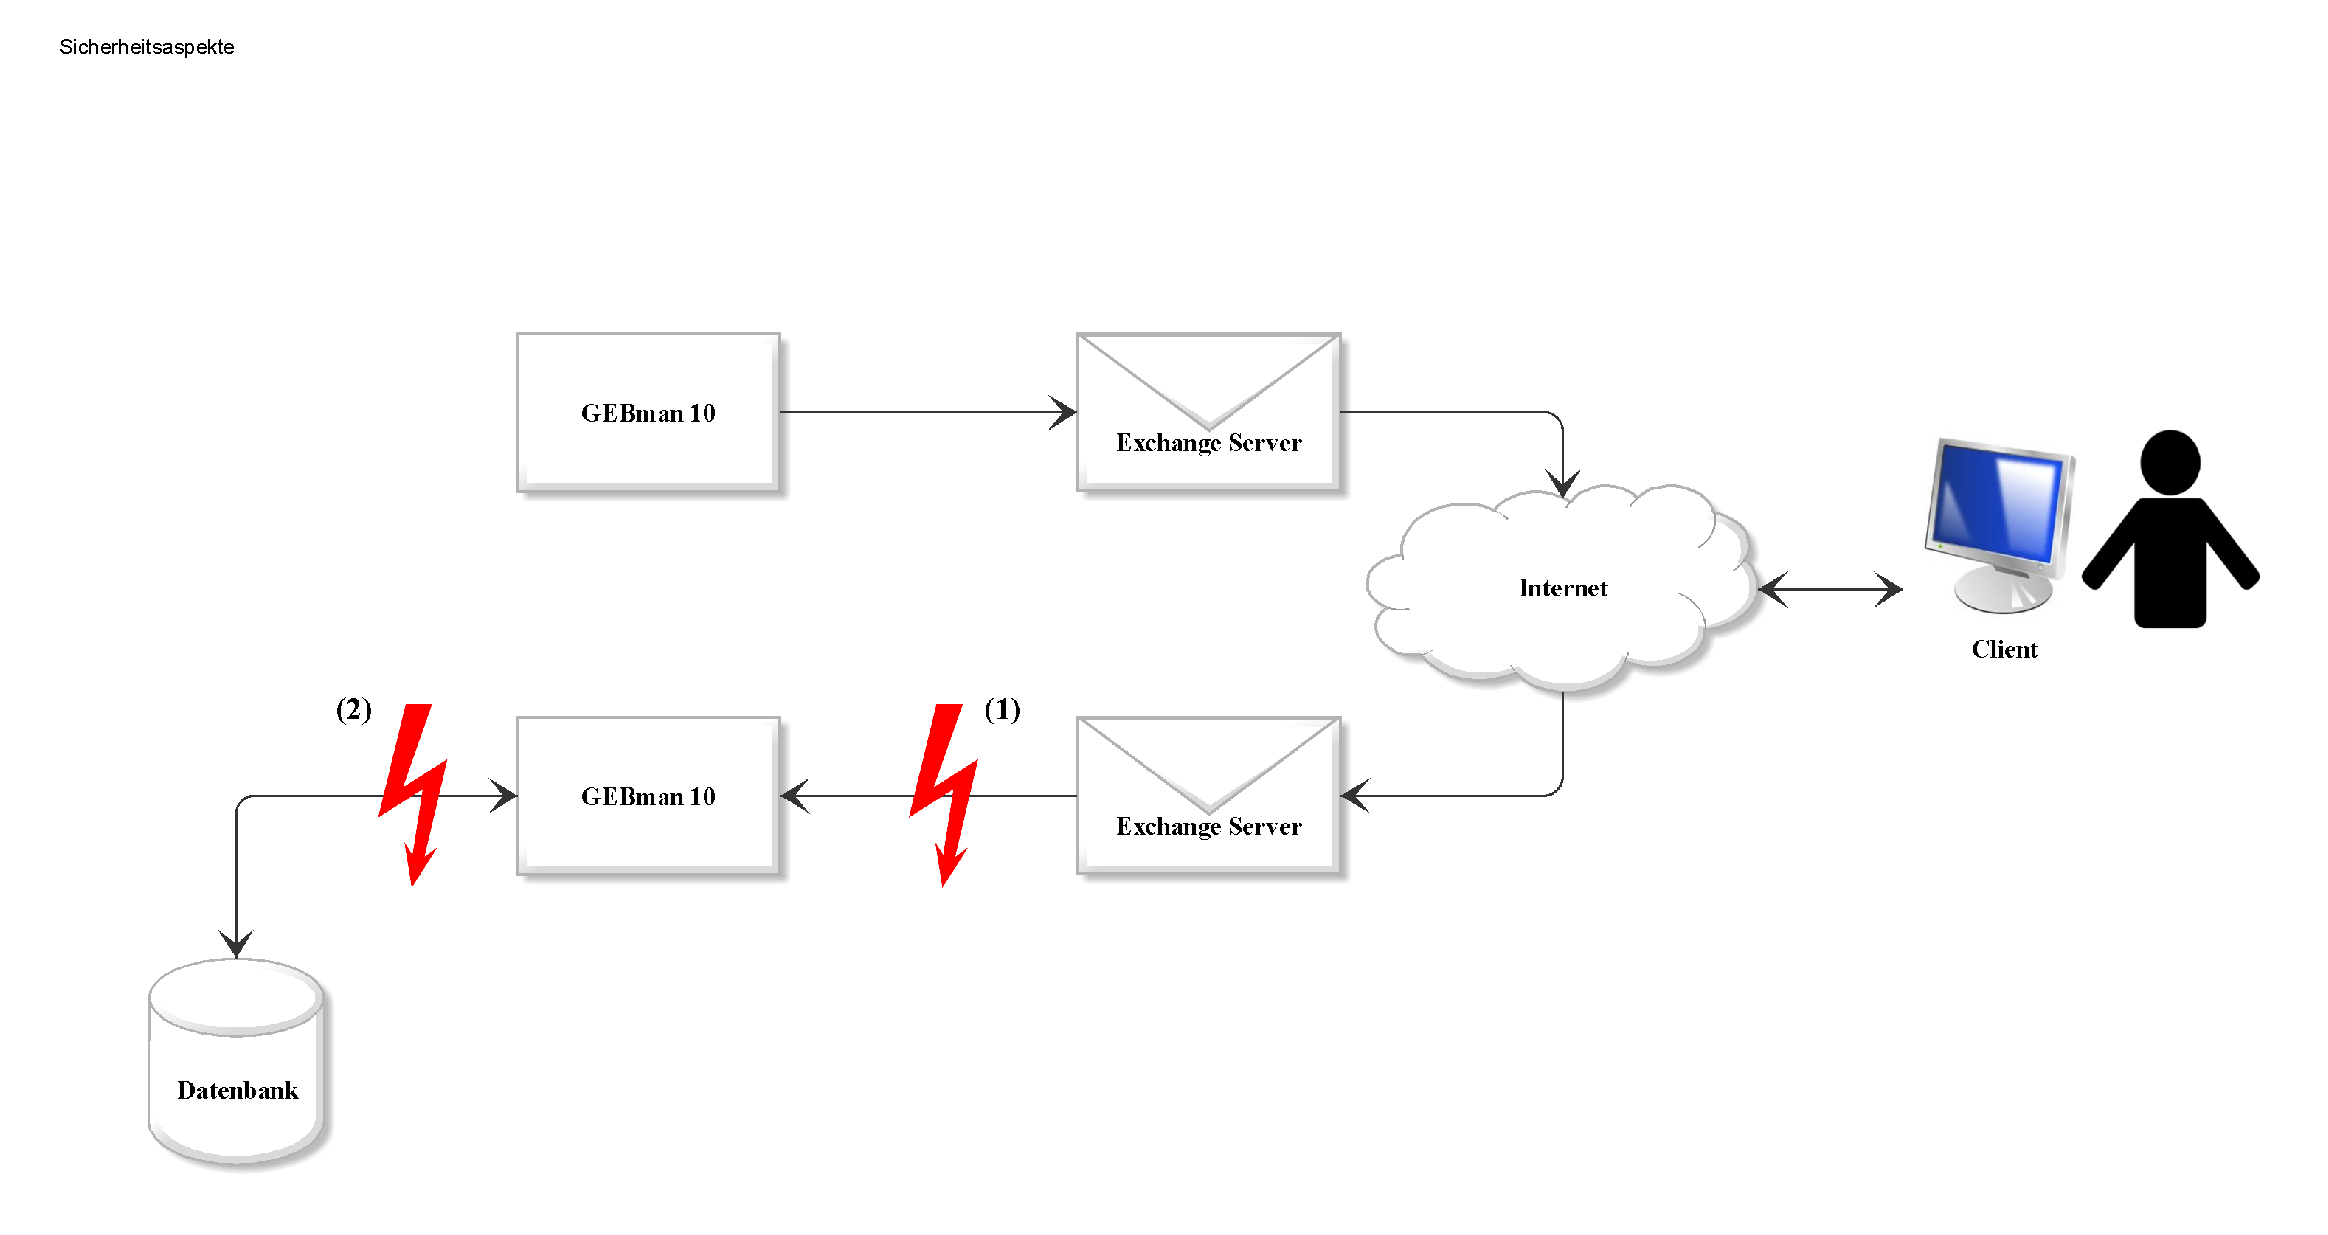
\includegraphics[width=0.85\textwidth]{Abbildungen/Sicherheitsaspekte.pdf}
	\caption[Sicherheitsprobleme]{Sicherheitsprobleme, Quelle: eigene Darstellung}
	\label{fig:Sicherheitsprobleme}
\end{figure}

\noindent
Der erste kritische Bereich - gekennzeichnet mit der (1) - symbolisiert das erste Problem. Sollte der Exchange Server mit E-Mails überhäuft werden, so wird für jede E-Mail eine neue Meldung in GEBman 10 angelegt. Das bedeutet, dass wenn pro Minute 100 E-Mails den Exchange Server erreichen, auch 100 Meldungen angelegt werden. Das würde das System deutlich verlangsamen, wenn nicht sogar zum Absturz bringen. Eine Möglichkeit, dieser Gefahrenquelle entgegenzutreten, ist, die Sender der E-Mails auszuschließen, sobald diese eine ungewöhnlich hohe Anzahl an E-Mails versenden. Dadurch würden dann die E-Mails von dem Benutzer nicht ausgelesen werden, alle anderen E-Mails jedoch schon.\\

\noindent
Bei dem zweiten kritischen Bereich der Abbildung~\ref{fig:Sicherheitsprobleme} - gekennzeichnet mit der (2) - muss auf die Speicherung der Daten in der Datenbank geachtet werden. GEBman 10 synchronisiert in regelmäßigen Abständen die Nachrichten vom hinterlegten Exchange Server. Entsprechend ihrer ID werden die Nachrichten in der Datenbank von GEBman 10 gespeichert. Nun könnte ein Angreifer beispielsweise versuchen, in den Textkörper der E-Mail JavaScript-Code oder HTML Befehle einzubetten. Diese Angriffsmethode nennt sich Cross-Site-Scripting (XSS). Gelangt nun ein Benutzer auf die Seite, auf der dieser XSS-Code injiziert wurde, könnten Informationen preisgegeben und versendet werden, auf die es der Angreifer abgesehen hat.\footnote{Vgl. \citeauthor{Rohr} (\citeyear{Rohr}), S. 90ff.}\newline
Es wäre möglich, den Textkörper und den Betreff einer E-Mail zu prüfen, bevor diese in der Datenbank gespeichert wird. Jedoch ist das nicht nötig, da GEBman 10 über spezielle Abwehrmechanismen verfügt, die das Injizieren von XSS-Code nutzlos macht und somit keine Gefahr für einen Benutzer darstellt.

 

